\documentclass[]{book}
\usepackage{lmodern}
\usepackage{amssymb,amsmath}
\usepackage{ifxetex,ifluatex}
\usepackage{fixltx2e} % provides \textsubscript
\ifnum 0\ifxetex 1\fi\ifluatex 1\fi=0 % if pdftex
  \usepackage[T1]{fontenc}
  \usepackage[utf8]{inputenc}
\else % if luatex or xelatex
  \ifxetex
    \usepackage{mathspec}
  \else
    \usepackage{fontspec}
  \fi
  \defaultfontfeatures{Ligatures=TeX,Scale=MatchLowercase}
\fi
% use upquote if available, for straight quotes in verbatim environments
\IfFileExists{upquote.sty}{\usepackage{upquote}}{}
% use microtype if available
\IfFileExists{microtype.sty}{%
\usepackage{microtype}
\UseMicrotypeSet[protrusion]{basicmath} % disable protrusion for tt fonts
}{}
\usepackage{hyperref}
\hypersetup{unicode=true,
            pdftitle={数据分析内功心法},
            pdfauthor={Genowis},
            pdfborder={0 0 0},
            breaklinks=true}
\urlstyle{same}  % don't use monospace font for urls
\usepackage{natbib}
\bibliographystyle{apalike}
\usepackage{color}
\usepackage{fancyvrb}
\newcommand{\VerbBar}{|}
\newcommand{\VERB}{\Verb[commandchars=\\\{\}]}
\DefineVerbatimEnvironment{Highlighting}{Verbatim}{commandchars=\\\{\}}
% Add ',fontsize=\small' for more characters per line
\usepackage{framed}
\definecolor{shadecolor}{RGB}{248,248,248}
\newenvironment{Shaded}{\begin{snugshade}}{\end{snugshade}}
\newcommand{\AlertTok}[1]{\textcolor[rgb]{0.94,0.16,0.16}{#1}}
\newcommand{\AnnotationTok}[1]{\textcolor[rgb]{0.56,0.35,0.01}{\textbf{\textit{#1}}}}
\newcommand{\AttributeTok}[1]{\textcolor[rgb]{0.77,0.63,0.00}{#1}}
\newcommand{\BaseNTok}[1]{\textcolor[rgb]{0.00,0.00,0.81}{#1}}
\newcommand{\BuiltInTok}[1]{#1}
\newcommand{\CharTok}[1]{\textcolor[rgb]{0.31,0.60,0.02}{#1}}
\newcommand{\CommentTok}[1]{\textcolor[rgb]{0.56,0.35,0.01}{\textit{#1}}}
\newcommand{\CommentVarTok}[1]{\textcolor[rgb]{0.56,0.35,0.01}{\textbf{\textit{#1}}}}
\newcommand{\ConstantTok}[1]{\textcolor[rgb]{0.00,0.00,0.00}{#1}}
\newcommand{\ControlFlowTok}[1]{\textcolor[rgb]{0.13,0.29,0.53}{\textbf{#1}}}
\newcommand{\DataTypeTok}[1]{\textcolor[rgb]{0.13,0.29,0.53}{#1}}
\newcommand{\DecValTok}[1]{\textcolor[rgb]{0.00,0.00,0.81}{#1}}
\newcommand{\DocumentationTok}[1]{\textcolor[rgb]{0.56,0.35,0.01}{\textbf{\textit{#1}}}}
\newcommand{\ErrorTok}[1]{\textcolor[rgb]{0.64,0.00,0.00}{\textbf{#1}}}
\newcommand{\ExtensionTok}[1]{#1}
\newcommand{\FloatTok}[1]{\textcolor[rgb]{0.00,0.00,0.81}{#1}}
\newcommand{\FunctionTok}[1]{\textcolor[rgb]{0.00,0.00,0.00}{#1}}
\newcommand{\ImportTok}[1]{#1}
\newcommand{\InformationTok}[1]{\textcolor[rgb]{0.56,0.35,0.01}{\textbf{\textit{#1}}}}
\newcommand{\KeywordTok}[1]{\textcolor[rgb]{0.13,0.29,0.53}{\textbf{#1}}}
\newcommand{\NormalTok}[1]{#1}
\newcommand{\OperatorTok}[1]{\textcolor[rgb]{0.81,0.36,0.00}{\textbf{#1}}}
\newcommand{\OtherTok}[1]{\textcolor[rgb]{0.56,0.35,0.01}{#1}}
\newcommand{\PreprocessorTok}[1]{\textcolor[rgb]{0.56,0.35,0.01}{\textit{#1}}}
\newcommand{\RegionMarkerTok}[1]{#1}
\newcommand{\SpecialCharTok}[1]{\textcolor[rgb]{0.00,0.00,0.00}{#1}}
\newcommand{\SpecialStringTok}[1]{\textcolor[rgb]{0.31,0.60,0.02}{#1}}
\newcommand{\StringTok}[1]{\textcolor[rgb]{0.31,0.60,0.02}{#1}}
\newcommand{\VariableTok}[1]{\textcolor[rgb]{0.00,0.00,0.00}{#1}}
\newcommand{\VerbatimStringTok}[1]{\textcolor[rgb]{0.31,0.60,0.02}{#1}}
\newcommand{\WarningTok}[1]{\textcolor[rgb]{0.56,0.35,0.01}{\textbf{\textit{#1}}}}
\usepackage{longtable,booktabs}
\usepackage{graphicx,grffile}
\makeatletter
\def\maxwidth{\ifdim\Gin@nat@width>\linewidth\linewidth\else\Gin@nat@width\fi}
\def\maxheight{\ifdim\Gin@nat@height>\textheight\textheight\else\Gin@nat@height\fi}
\makeatother
% Scale images if necessary, so that they will not overflow the page
% margins by default, and it is still possible to overwrite the defaults
% using explicit options in \includegraphics[width, height, ...]{}
\setkeys{Gin}{width=\maxwidth,height=\maxheight,keepaspectratio}
\IfFileExists{parskip.sty}{%
\usepackage{parskip}
}{% else
\setlength{\parindent}{0pt}
\setlength{\parskip}{6pt plus 2pt minus 1pt}
}
\setlength{\emergencystretch}{3em}  % prevent overfull lines
\providecommand{\tightlist}{%
  \setlength{\itemsep}{0pt}\setlength{\parskip}{0pt}}
\setcounter{secnumdepth}{5}
% Redefines (sub)paragraphs to behave more like sections
\ifx\paragraph\undefined\else
\let\oldparagraph\paragraph
\renewcommand{\paragraph}[1]{\oldparagraph{#1}\mbox{}}
\fi
\ifx\subparagraph\undefined\else
\let\oldsubparagraph\subparagraph
\renewcommand{\subparagraph}[1]{\oldsubparagraph{#1}\mbox{}}
\fi

%%% Use protect on footnotes to avoid problems with footnotes in titles
\let\rmarkdownfootnote\footnote%
\def\footnote{\protect\rmarkdownfootnote}

%%% Change title format to be more compact
\usepackage{titling}

% Create subtitle command for use in maketitle
\providecommand{\subtitle}[1]{
  \posttitle{
    \begin{center}\large#1\end{center}
    }
}

\setlength{\droptitle}{-2em}

  \title{数据分析内功心法}
    \pretitle{\vspace{\droptitle}\centering\huge}
  \posttitle{\par}
    \author{Genowis}
    \preauthor{\centering\large\emph}
  \postauthor{\par}
      \predate{\centering\large\emph}
  \postdate{\par}
    \date{2019-09-23}

\usepackage{booktabs}

\begin{document}
\maketitle

{
\setcounter{tocdepth}{1}
\tableofcontents
}
\hypertarget{section}{%
\chapter{前言}\label{section}}

本教程主要介绍数据分析中常用的方法和工具,特别是R语言常用的框架和基本操作。相关读者应将本书作为基础性介绍,而非一个完整的工具说明文档。读者如果想进一步学习相关方向,需要查阅相关文档,github和Stack Overflow,或者咨询其他有经验的人员。

注意:

\begin{itemize}
\tightlist
\item
  教程中给出的一些论断,均基于当前的工作实践和R的开发状况,因此无法做到完全的与时俱进和全面认知,请读者发挥主观能动性,发现新的认知。
\item
  一些信息来自于网络,作为内部教程不再单独说明。
\end{itemize}

\hypertarget{intro}{%
\chapter{R环境介绍}\label{intro}}

\hypertarget{section-1}{%
\section{相关历史}\label{section-1}}

\begin{quote}
R is a language and environment for statistical computing and graphics. It is a GNU project which is similar to the S language and environment which was developed at Bell Laboratories (formerly AT\&T, now Lucent Technologies) by John Chambers and colleagues.
\end{quote}

\begin{itemize}
\tightlist
\item
  1980年,源于S语言,新西兰奥克兰大学
\item
  统计计算和图形化
\end{itemize}

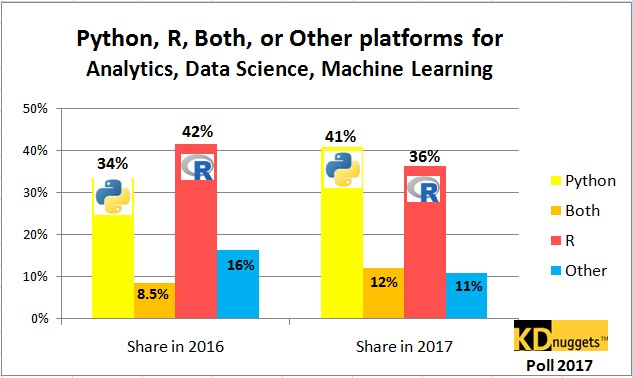
\includegraphics{figures/poll.jpg}

\begin{center}\rule{0.5\linewidth}{\linethickness}\end{center}

优点:

\begin{itemize}
\tightlist
\item
  免费,开源
\item
  面向统计分析
\item
  简单易学
\item
  可视化非常好
\item
  完整生态的开发流程
\item
  社区逐渐扩大
\end{itemize}

缺点:

\begin{itemize}
\tightlist
\item
  基于缓存的数据加载
\item
  运算效率第,对超大数据支持不力
\item
  国内普及度不高
\end{itemize}

\hypertarget{section-2}{%
\section{编程环境}\label{section-2}}

\begin{itemize}
\tightlist
\item
  Rstudio
\end{itemize}

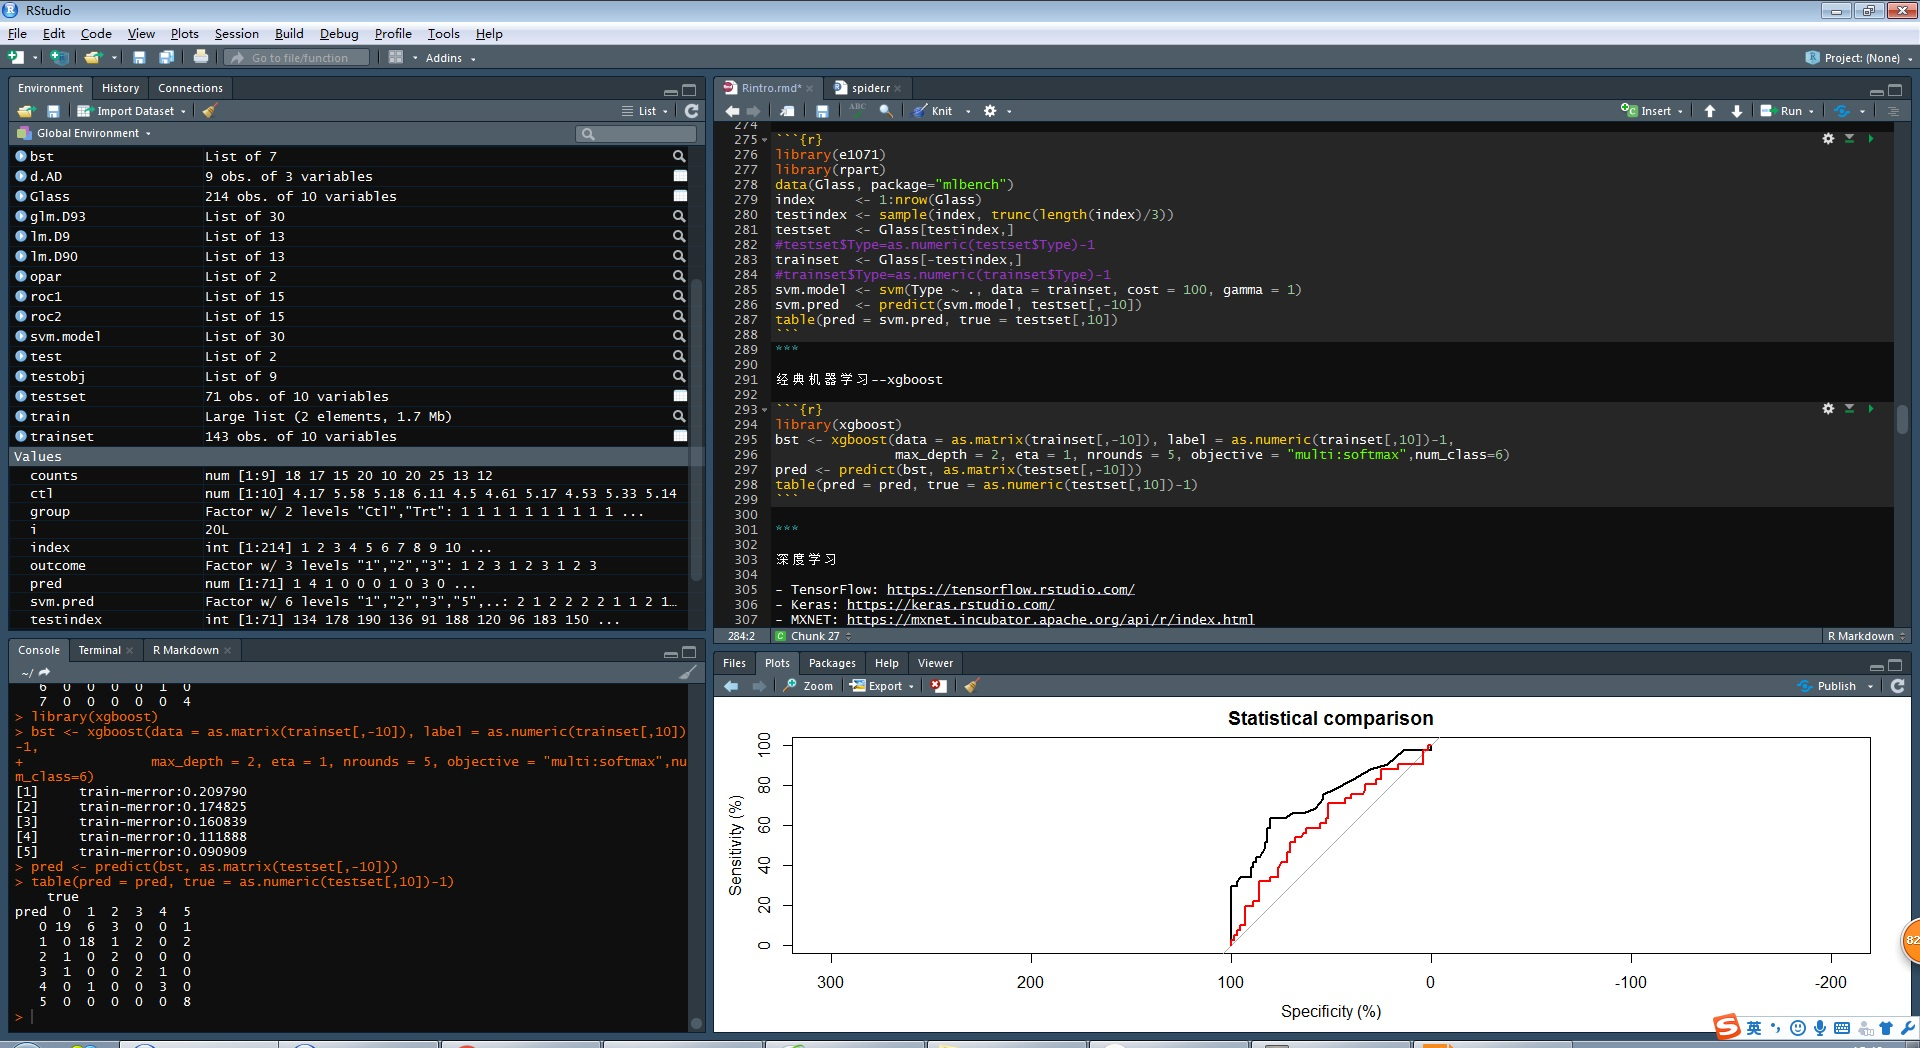
\includegraphics{figures/rstudio.jpg}

相关\href{https://www.rstudio.com/products/RStudio/}{连接}

\begin{center}\rule{0.5\linewidth}{\linethickness}\end{center}

\begin{itemize}
\tightlist
\item
  Jupyter
\end{itemize}

\begin{verbatim}
conda install -c r r-essentials
\end{verbatim}

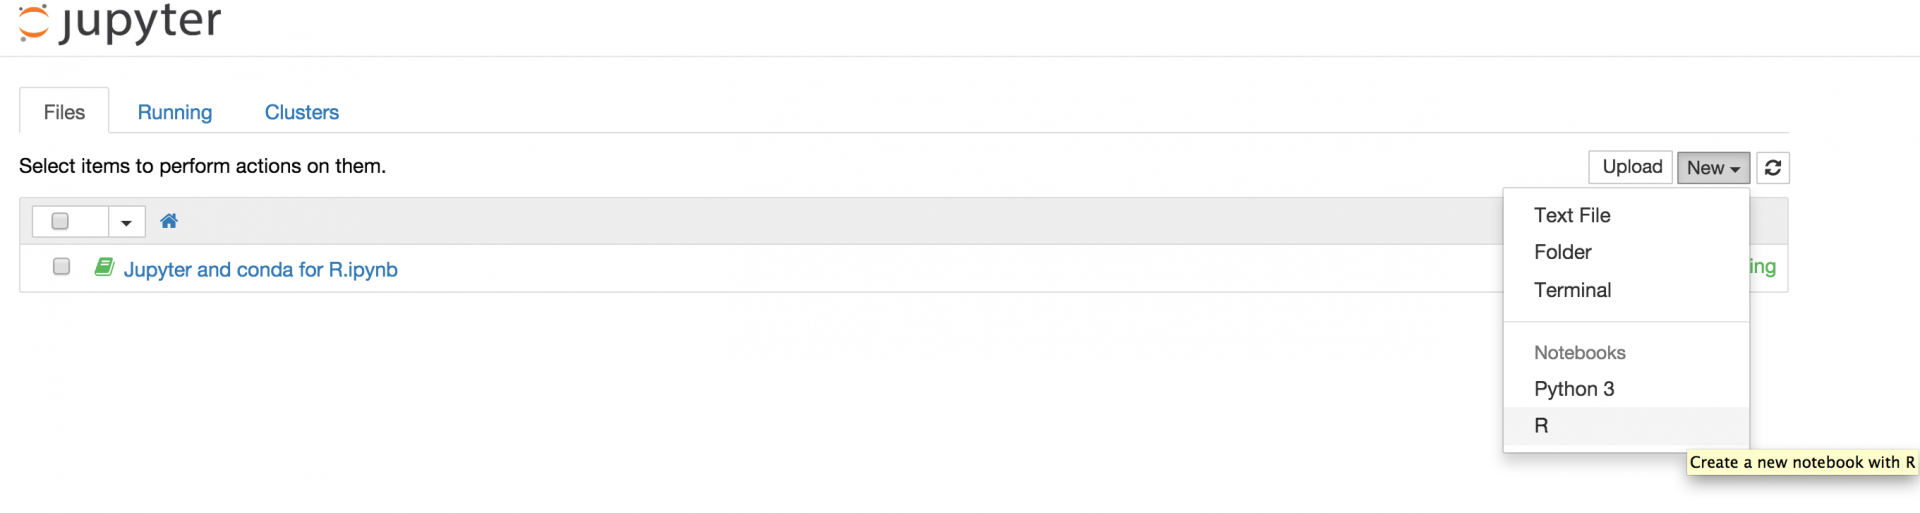
\includegraphics{figures/jupyter.png}

相关\href{https://www.anaconda.com/developer-blog/jupyter-and-conda-r/}{连接}

\hypertarget{section-3}{%
\section{数据类型}\label{section-3}}

\begin{itemize}
\tightlist
\item
  字符型
\item
  数值型
\item
  整数型
\item
  日期类型
\item
  逻辑型
\end{itemize}

\begin{Shaded}
\begin{Highlighting}[]
\OperatorTok{-}\StringTok{ }\NormalTok{字符character}\OperatorTok{:}\StringTok{ "a"}\NormalTok{, }\StringTok{"1"}\NormalTok{, }\StringTok{"apple"}\NormalTok{, }\StringTok{"@"}
\end{Highlighting}
\end{Shaded}

\begin{Shaded}
\begin{Highlighting}[]
\OperatorTok{-}\StringTok{ }\NormalTok{数值numeric}\OperatorTok{:}\StringTok{ }\DecValTok{1}\NormalTok{, }\FloatTok{3.14}\NormalTok{, }\DecValTok{100}\NormalTok{, }\FloatTok{2e10}
\end{Highlighting}
\end{Shaded}

\begin{Shaded}
\begin{Highlighting}[]
\OperatorTok{-}\StringTok{ }\NormalTok{整数integer}\OperatorTok{:}\StringTok{ }\DecValTok{1}\NormalTok{, }\DecValTok{2}\NormalTok{, }\DecValTok{500}
\end{Highlighting}
\end{Shaded}

\begin{Shaded}
\begin{Highlighting}[]
\OperatorTok{-}\StringTok{ }\NormalTok{因子factor}\OperatorTok{:}\StringTok{ }\NormalTok{肝细胞癌(1),肝内胆管癌(2)}
\end{Highlighting}
\end{Shaded}

\begin{Shaded}
\begin{Highlighting}[]
\OperatorTok{-}\StringTok{ }\NormalTok{逻辑logical}\OperatorTok{:}\StringTok{ }\OtherTok{TRUE}\NormalTok{, }\OtherTok{FALSE}
\end{Highlighting}
\end{Shaded}

\begin{Shaded}
\begin{Highlighting}[]
\OperatorTok{-}\StringTok{ }\NormalTok{日期date}\OperatorTok{:}\StringTok{ }\DecValTok{2018-01-19}\NormalTok{, }\DecValTok{19}\OperatorTok{/}\DecValTok{1}\OperatorTok{/}\DecValTok{2018}
\end{Highlighting}
\end{Shaded}

\hypertarget{section-4}{%
\section{数据结构}\label{section-4}}

\begin{itemize}
\tightlist
\item
  因子
\item
  向量
\item
  列表
\item
  矩阵
\item
  数据框
\end{itemize}

\begin{Shaded}
\begin{Highlighting}[]
\OperatorTok{-}\StringTok{ }\NormalTok{向量vector}\OperatorTok{:}\StringTok{ }\KeywordTok{c}\NormalTok{(}\DecValTok{1}\NormalTok{,}\DecValTok{2}\NormalTok{,}\DecValTok{3}\NormalTok{),}\KeywordTok{c}\NormalTok{(}\StringTok{"a"}\NormalTok{,}\StringTok{"b"}\NormalTok{,}\StringTok{"c"}\NormalTok{), }\DecValTok{1}\OperatorTok{:}\DecValTok{10}
\end{Highlighting}
\end{Shaded}

\begin{Shaded}
\begin{Highlighting}[]
\OperatorTok{-}\StringTok{ }\NormalTok{列表list}\OperatorTok{:}\StringTok{ }\KeywordTok{list}\NormalTok{(}\DecValTok{1}\NormalTok{,}\DecValTok{2}\NormalTok{,}\DecValTok{3}\NormalTok{),}\KeywordTok{list}\NormalTok{(}\DataTypeTok{a=}\StringTok{"A"}\NormalTok{,}\DataTypeTok{b=}\StringTok{"B"}\NormalTok{,}\DataTypeTok{c=}\StringTok{"C"}\NormalTok{,}\DataTypeTok{d=}\DecValTok{1}\NormalTok{)}
\end{Highlighting}
\end{Shaded}

\begin{Shaded}
\begin{Highlighting}[]
\OperatorTok{-}\StringTok{ }\NormalTok{矩阵}\OperatorTok{/}\NormalTok{数组matrix}\OperatorTok{/}\NormalTok{array}\OperatorTok{:}\StringTok{ }\KeywordTok{matrix}\NormalTok{(}\KeywordTok{c}\NormalTok{(}\DecValTok{1}\NormalTok{,}\DecValTok{2}\NormalTok{,}\DecValTok{3}\NormalTok{,}\DecValTok{4}\NormalTok{),}\DataTypeTok{ncol=}\DecValTok{2}\NormalTok{)}
\end{Highlighting}
\end{Shaded}

\begin{Shaded}
\begin{Highlighting}[]
\OperatorTok{-}\StringTok{ }\NormalTok{数据框data.frame}\OperatorTok{:}\StringTok{ }\KeywordTok{data.frame}\NormalTok{(}\DataTypeTok{ID=}\KeywordTok{c}\NormalTok{(}\DecValTok{1}\NormalTok{,}\DecValTok{2}\NormalTok{,}\DecValTok{3}\NormalTok{), 血型=}\KeywordTok{c}\NormalTok{(}\StringTok{"A"}\NormalTok{,}\StringTok{"B"}\NormalTok{,}\StringTok{"A"}\NormalTok{))}
\end{Highlighting}
\end{Shaded}

\hypertarget{section-5}{%
\section{控制}\label{section-5}}

\begin{itemize}
\tightlist
\item
  for
\end{itemize}

\begin{Shaded}
\begin{Highlighting}[]
\ControlFlowTok{for}\NormalTok{ ( i }\ControlFlowTok{in} \DecValTok{1}\OperatorTok{:}\DecValTok{20}\NormalTok{) \{}
  
  \ControlFlowTok{if}\NormalTok{ (i }\OperatorTok\StringTok{ }\DecValTok{2}\OperatorTok{==}\DecValTok{0}\NormalTok{)\{}
    \KeywordTok{print}\NormalTok{(}\KeywordTok{paste}\NormalTok{(i,}\StringTok{"是偶数"}\NormalTok{,}\DataTypeTok{sep=}\StringTok{""}\NormalTok{))}
\NormalTok{  \}}
  \ControlFlowTok{else}\NormalTok{ \{}
    \ControlFlowTok{next}
\NormalTok{  \}}
\NormalTok{\}}
\end{Highlighting}
\end{Shaded}

\begin{verbatim}
## [1] "2是偶数"
## [1] "4是偶数"
## [1] "6是偶数"
## [1] "8是偶数"
## [1] "10是偶数"
## [1] "12是偶数"
## [1] "14是偶数"
## [1] "16是偶数"
## [1] "18是偶数"
## [1] "20是偶数"
\end{verbatim}

\begin{itemize}
\tightlist
\item
  if\ldots{} else
\item
  while\ldots{}
\item
  repeat
\item
  break
\item
  next
\end{itemize}

\hypertarget{section-6}{%
\section{函数}\label{section-6}}

\begin{Shaded}
\begin{Highlighting}[]
\OperatorTok{-}\StringTok{ }\NormalTok{函数名:}\KeywordTok{mean}\NormalTok{(), }\KeywordTok{get_IHC}\NormalTok{()}
\end{Highlighting}
\end{Shaded}

\begin{Shaded}
\begin{Highlighting}[]
\OperatorTok{-}\StringTok{ }\NormalTok{函数体}\OperatorTok{:}\StringTok{ }\NormalTok{通过}\KeywordTok{body}\NormalTok{(函数名)查看}
\end{Highlighting}
\end{Shaded}

\begin{Shaded}
\begin{Highlighting}[]
\OperatorTok{-}\StringTok{ }\NormalTok{参数:}\KeywordTok{get_IHC}\NormalTok{(x, y) 其中x表示文本,y表示要提取的IHC指标}
\end{Highlighting}
\end{Shaded}

\hypertarget{section-7}{%
\section{基本语法}\label{section-7}}

\begin{Shaded}
\begin{Highlighting}[]
\NormalTok{函数名=}\ControlFlowTok{function}\NormalTok{(参数)\{}
\NormalTok{  运算逻辑}
\NormalTok{\}}
\end{Highlighting}
\end{Shaded}

\begin{Shaded}
\begin{Highlighting}[]
\NormalTok{func=}\ControlFlowTok{function}\NormalTok{(x,y)\{}
  \KeywordTok{return}\NormalTok{(x}\OperatorTok{/}\NormalTok{(y}\OperatorTok{+}\DecValTok{1}\NormalTok{))}
\NormalTok{\}}

\KeywordTok{func}\NormalTok{(}\DecValTok{1}\NormalTok{,}\DecValTok{1}\NormalTok{)}
\end{Highlighting}
\end{Shaded}

\begin{verbatim}
## [1] 0.5
\end{verbatim}

\hypertarget{section-8}{%
\section{绘图}\label{section-8}}

\hypertarget{base}{%
\section{base库中的常用函数}\label{base}}

\hypertarget{section-9}{%
\subsection{算数运算}\label{section-9}}

\begin{itemize}
\tightlist
\item
  +,*, /
\end{itemize}

\begin{Shaded}
\begin{Highlighting}[]
\DecValTok{1}\OperatorTok{:}\DecValTok{10}\OperatorTok{+}\DecValTok{2}
\end{Highlighting}
\end{Shaded}

\begin{verbatim}
##  [1]  3  4  5  6  7  8  9 10 11 12
\end{verbatim}

\begin{Shaded}
\begin{Highlighting}[]
\DecValTok{9}\OperatorTok{/}\NormalTok{(}\DecValTok{1}\OperatorTok{:}\DecValTok{3}\NormalTok{)}\OperatorTok{-}\FloatTok{0.5}
\end{Highlighting}
\end{Shaded}

\begin{verbatim}
## [1] 8.5 4.0 2.5
\end{verbatim}

\hypertarget{section-10}{%
\subsection{统计运算}\label{section-10}}

\begin{itemize}
\tightlist
\item
  mean(),max(),min(),quantile(),sum(),summary()
\end{itemize}

\begin{Shaded}
\begin{Highlighting}[]
\KeywordTok{summary}\NormalTok{(}\KeywordTok{rnorm}\NormalTok{(}\DecValTok{100}\NormalTok{))}
\end{Highlighting}
\end{Shaded}

\begin{verbatim}
##      Min.   1st Qu.    Median      Mean   3rd Qu.      Max. 
## -2.518890 -0.486208  0.191744  0.008009  0.783987  1.628505
\end{verbatim}

\hypertarget{section-11}{%
\subsection{逻辑运算}\label{section-11}}

\begin{itemize}
\tightlist
\item
  \&, \textbar{}, !
\end{itemize}

\begin{Shaded}
\begin{Highlighting}[]
\OperatorTok{!}\NormalTok{(}\DecValTok{2}\OperatorTok{>}\DecValTok{1} \OperatorTok{|}\StringTok{ }\DecValTok{2}\OperatorTok{>}\DecValTok{3}\NormalTok{)}
\end{Highlighting}
\end{Shaded}

\begin{verbatim}
## [1] FALSE
\end{verbatim}

\hypertarget{section-12}{%
\subsection{字符串操作}\label{section-12}}

\begin{itemize}
\tightlist
\item
  paste(), grep(),grepl(), strsplit(), strsub()
\end{itemize}

\begin{Shaded}
\begin{Highlighting}[]
\NormalTok{tmp=}\KeywordTok{paste}\NormalTok{(}\KeywordTok{c}\NormalTok{(}\DecValTok{1}\OperatorTok{:}\DecValTok{10}\NormalTok{),}\StringTok{"163.com"}\NormalTok{,}\DataTypeTok{sep=}\StringTok{"@"}\NormalTok{)}
\KeywordTok{unlist}\NormalTok{(}\KeywordTok{strsplit}\NormalTok{(tmp,}\DataTypeTok{split=}\StringTok{"@"}\NormalTok{))[}\KeywordTok{seq}\NormalTok{(}\DecValTok{1}\NormalTok{,}\DecValTok{20}\NormalTok{,}\DecValTok{2}\NormalTok{)]}
\end{Highlighting}
\end{Shaded}

\begin{verbatim}
##  [1] "1"  "2"  "3"  "4"  "5"  "6"  "7"  "8"  "9"  "10"
\end{verbatim}

\hypertarget{section-13}{%
\subsection{数据表操作}\label{section-13}}

\begin{itemize}
\tightlist
\item
  subset(), merge(), dim(), names()
\end{itemize}

\begin{Shaded}
\begin{Highlighting}[]
\NormalTok{df=}\KeywordTok{data.frame}\NormalTok{(}\DataTypeTok{x=}\DecValTok{1}\OperatorTok{:}\DecValTok{10}\NormalTok{,}\DataTypeTok{y=}\KeywordTok{rep}\NormalTok{(}\StringTok{"a"}\NormalTok{,}\DecValTok{10}\NormalTok{),}\DataTypeTok{stringsAsFactors =}\NormalTok{ F)}
\KeywordTok{dim}\NormalTok{(}\KeywordTok{subset}\NormalTok{(df,x}\OperatorTok{>}\DecValTok{5}\NormalTok{))}
\end{Highlighting}
\end{Shaded}

\begin{verbatim}
## [1] 5 2
\end{verbatim}

\hypertarget{section-14}{%
\subsection{绘图命令}\label{section-14}}

\begin{itemize}
\tightlist
\item
  plot(),adline(),hist()
\end{itemize}

\begin{Shaded}
\begin{Highlighting}[]
\KeywordTok{hist}\NormalTok{(}\KeywordTok{rnorm}\NormalTok{(}\DecValTok{100}\NormalTok{))}
\KeywordTok{abline}\NormalTok{(}\DataTypeTok{a=}\DecValTok{15}\NormalTok{,}\DataTypeTok{b=}\DecValTok{0}\NormalTok{)}
\end{Highlighting}
\end{Shaded}

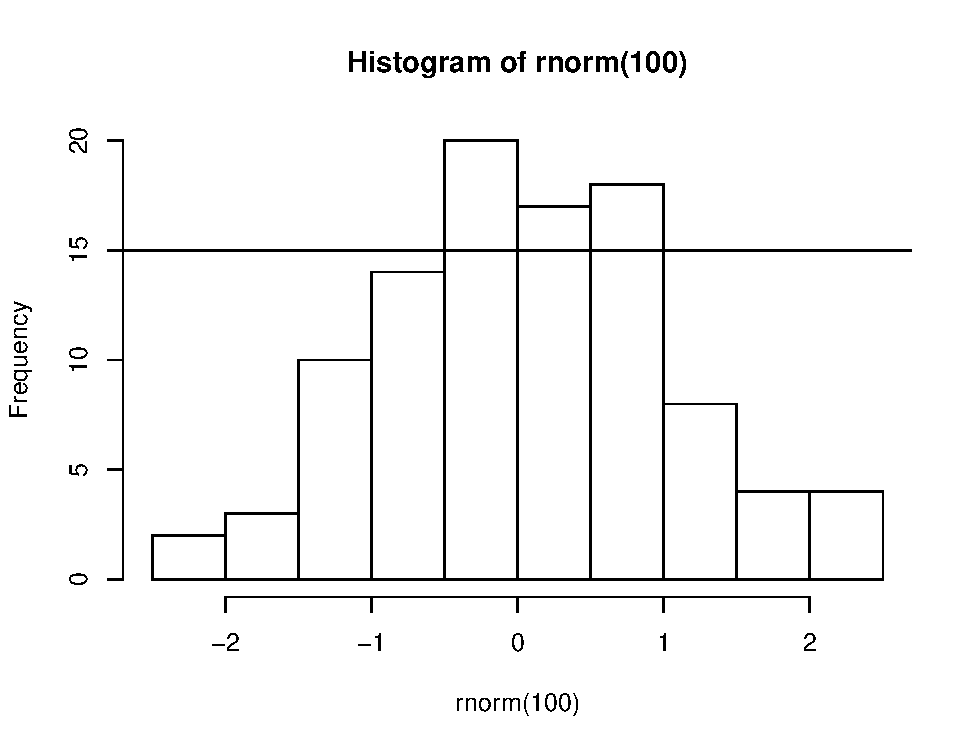
\includegraphics{DataAnalysisTutorial_files/figure-latex/unnamed-chunk-22-1.pdf}

\hypertarget{section-15}{%
\chapter{文件操作}\label{section-15}}

\hypertarget{section-16}{%
\section{表格文件}\label{section-16}}

\hypertarget{json}{%
\section{序列化json}\label{json}}

\hypertarget{html}{%
\section{爬虫html}\label{html}}

Here is a review of existing methods.

\hypertarget{section-17}{%
\chapter{统计分析}\label{section-17}}

\hypertarget{section-18}{%
\section{描述性统计}\label{section-18}}

\hypertarget{section-19}{%
\subsection{分位数}\label{section-19}}

\hypertarget{section-20}{%
\subsection{频度}\label{section-20}}

\hypertarget{section-21}{%
\subsection{置信度}\label{section-21}}

\hypertarget{section-22}{%
\section{相关性分析}\label{section-22}}

\hypertarget{section-23}{%
\subsection{相关系数}\label{section-23}}

\hypertarget{chi2}{%
\subsection{\texorpdfstring{\(\chi^2\)}{\textbackslash{}chi\^{}2}}\label{chi2}}

\hypertarget{section-24}{%
\section{假设检验}\label{section-24}}

\hypertarget{p}{%
\subsection{P值}\label{p}}

\hypertarget{section-25}{%
\subsection{常用检验方法}\label{section-25}}

\hypertarget{section-26}{%
\section{主成分分析}\label{section-26}}

\hypertarget{section-27}{%
\section{生存分析}\label{section-27}}

\hypertarget{section-28}{%
\chapter{数据操作}\label{section-28}}

\hypertarget{section-29}{%
\section{特殊数据类型操作}\label{section-29}}

\hypertarget{section-30}{%
\subsection{字符}\label{section-30}}

\hypertarget{section-31}{%
\subsection{日期/时间}\label{section-31}}

\hypertarget{json-1}{%
\subsection{json}\label{json-1}}

\hypertarget{xml}{%
\subsection{xml}\label{xml}}

\hypertarget{section-32}{%
\section{高效数据操作}\label{section-32}}

\hypertarget{data.table}{%
\subsection{data.table}\label{data.table}}

\hypertarget{plyrdplyr}{%
\subsection{plyr/dplyr}\label{plyrdplyr}}

\hypertarget{magrittr}{%
\subsection{magrittr}\label{magrittr}}

\hypertarget{section-33}{%
\chapter{可视化}\label{section-33}}

\hypertarget{section-34}{%
\section{基本原则}\label{section-34}}

\hypertarget{section-35}{%
\section{常用可视化包}\label{section-35}}

\hypertarget{ggplot2}{%
\subsection{ggplot2}\label{ggplot2}}

\hypertarget{plotly}{%
\subsection{plotly}\label{plotly}}

\hypertarget{echats4r}{%
\subsection{echats4r}\label{echats4r}}

\hypertarget{section-36}{%
\chapter{文档编写}\label{section-36}}

\hypertarget{markdown}{%
\section{markdown语言}\label{markdown}}

\hypertarget{rmarkdown}{%
\section{Rmarkdown}\label{rmarkdown}}

\hypertarget{section-37}{%
\chapter{速查表}\label{section-37}}

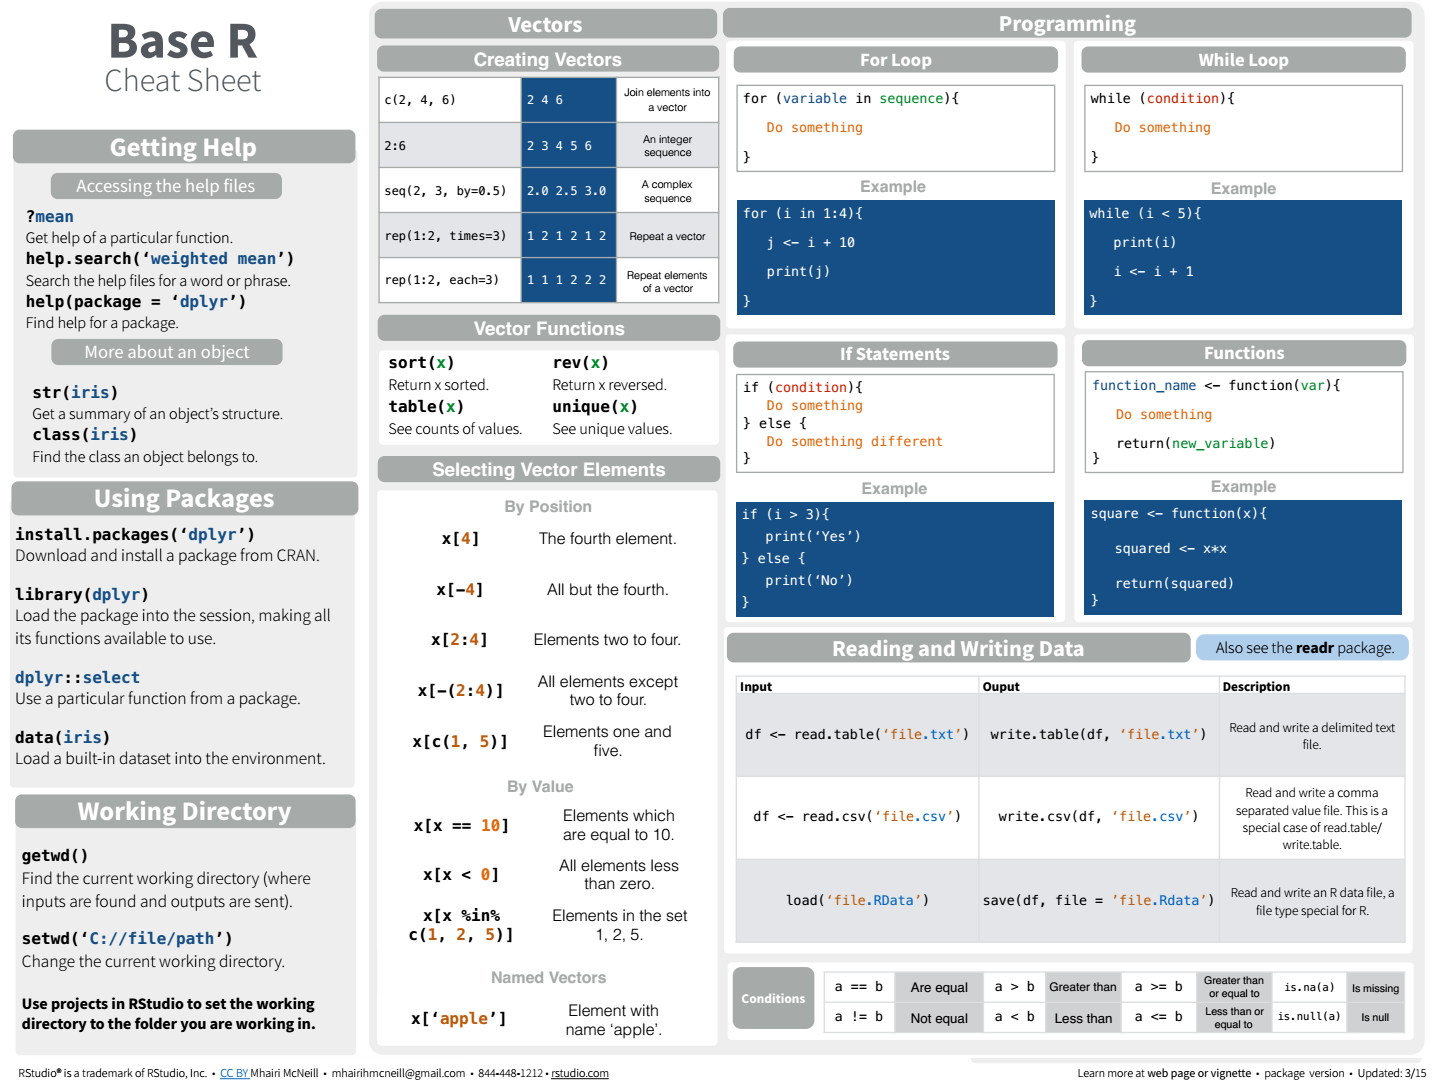
\includegraphics{figures/cheatsheet1.png}

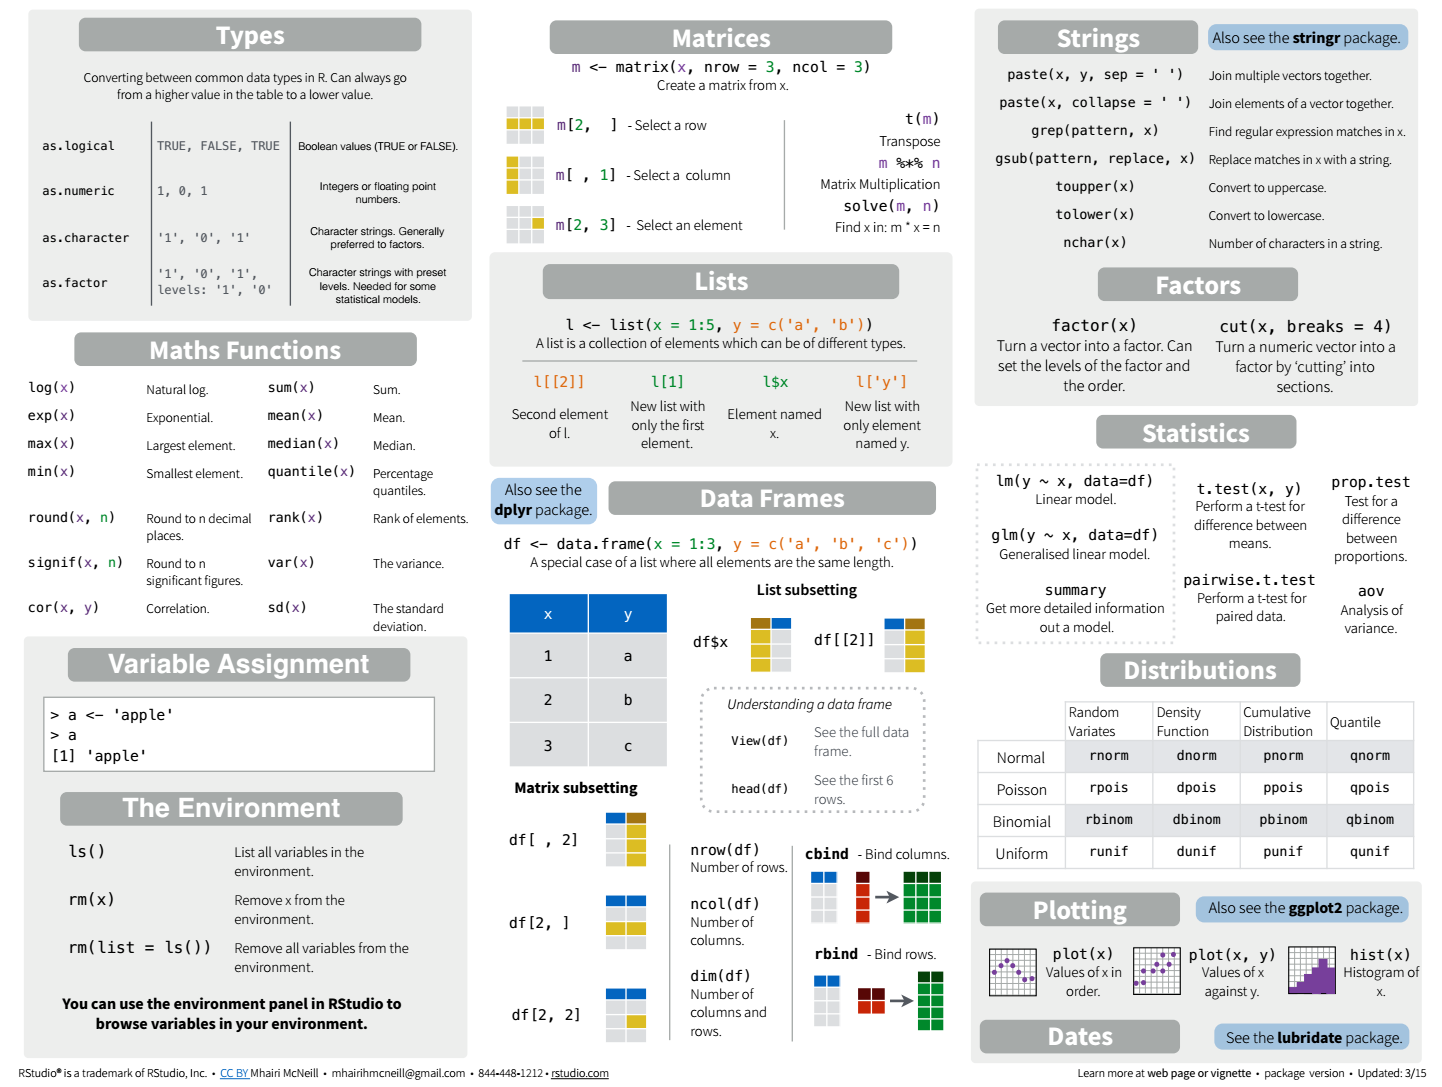
\includegraphics{figures/cheatsheet2.png}

\bibliography{book.bib,packages.bib}


\end{document}
